This chapter will explain how the system was implemented to make a correct web-based application. To make the application, I have used six various technologies such as HTML, CSS, JavaScript/jQuery, PHP, MySQL, and API to receive a message through the contact form. All the program was written in Sublime text editor.

\section{Front-End Development}
Front-end development is where developers convert the data to a graphical interface via HTML, CSS, and JavaScript so the user can view and interact with the site directly. I have made the front-end interesting where the user can read the information easily.

\subsection{HTML}
In order to make the front-end quicker, I have used a bootstrap 4 framework which will help me to design my site faster and easier. I have used this framework before in other so I know what tool and function to use to make my system interactive. Figure 4.1 shows the HTML code used on the site and has been taken from the index.php page. You can also see the bootstrap framework CDN in the head tag which imports the library in my system.

\begin{figure}[H]
\centering
    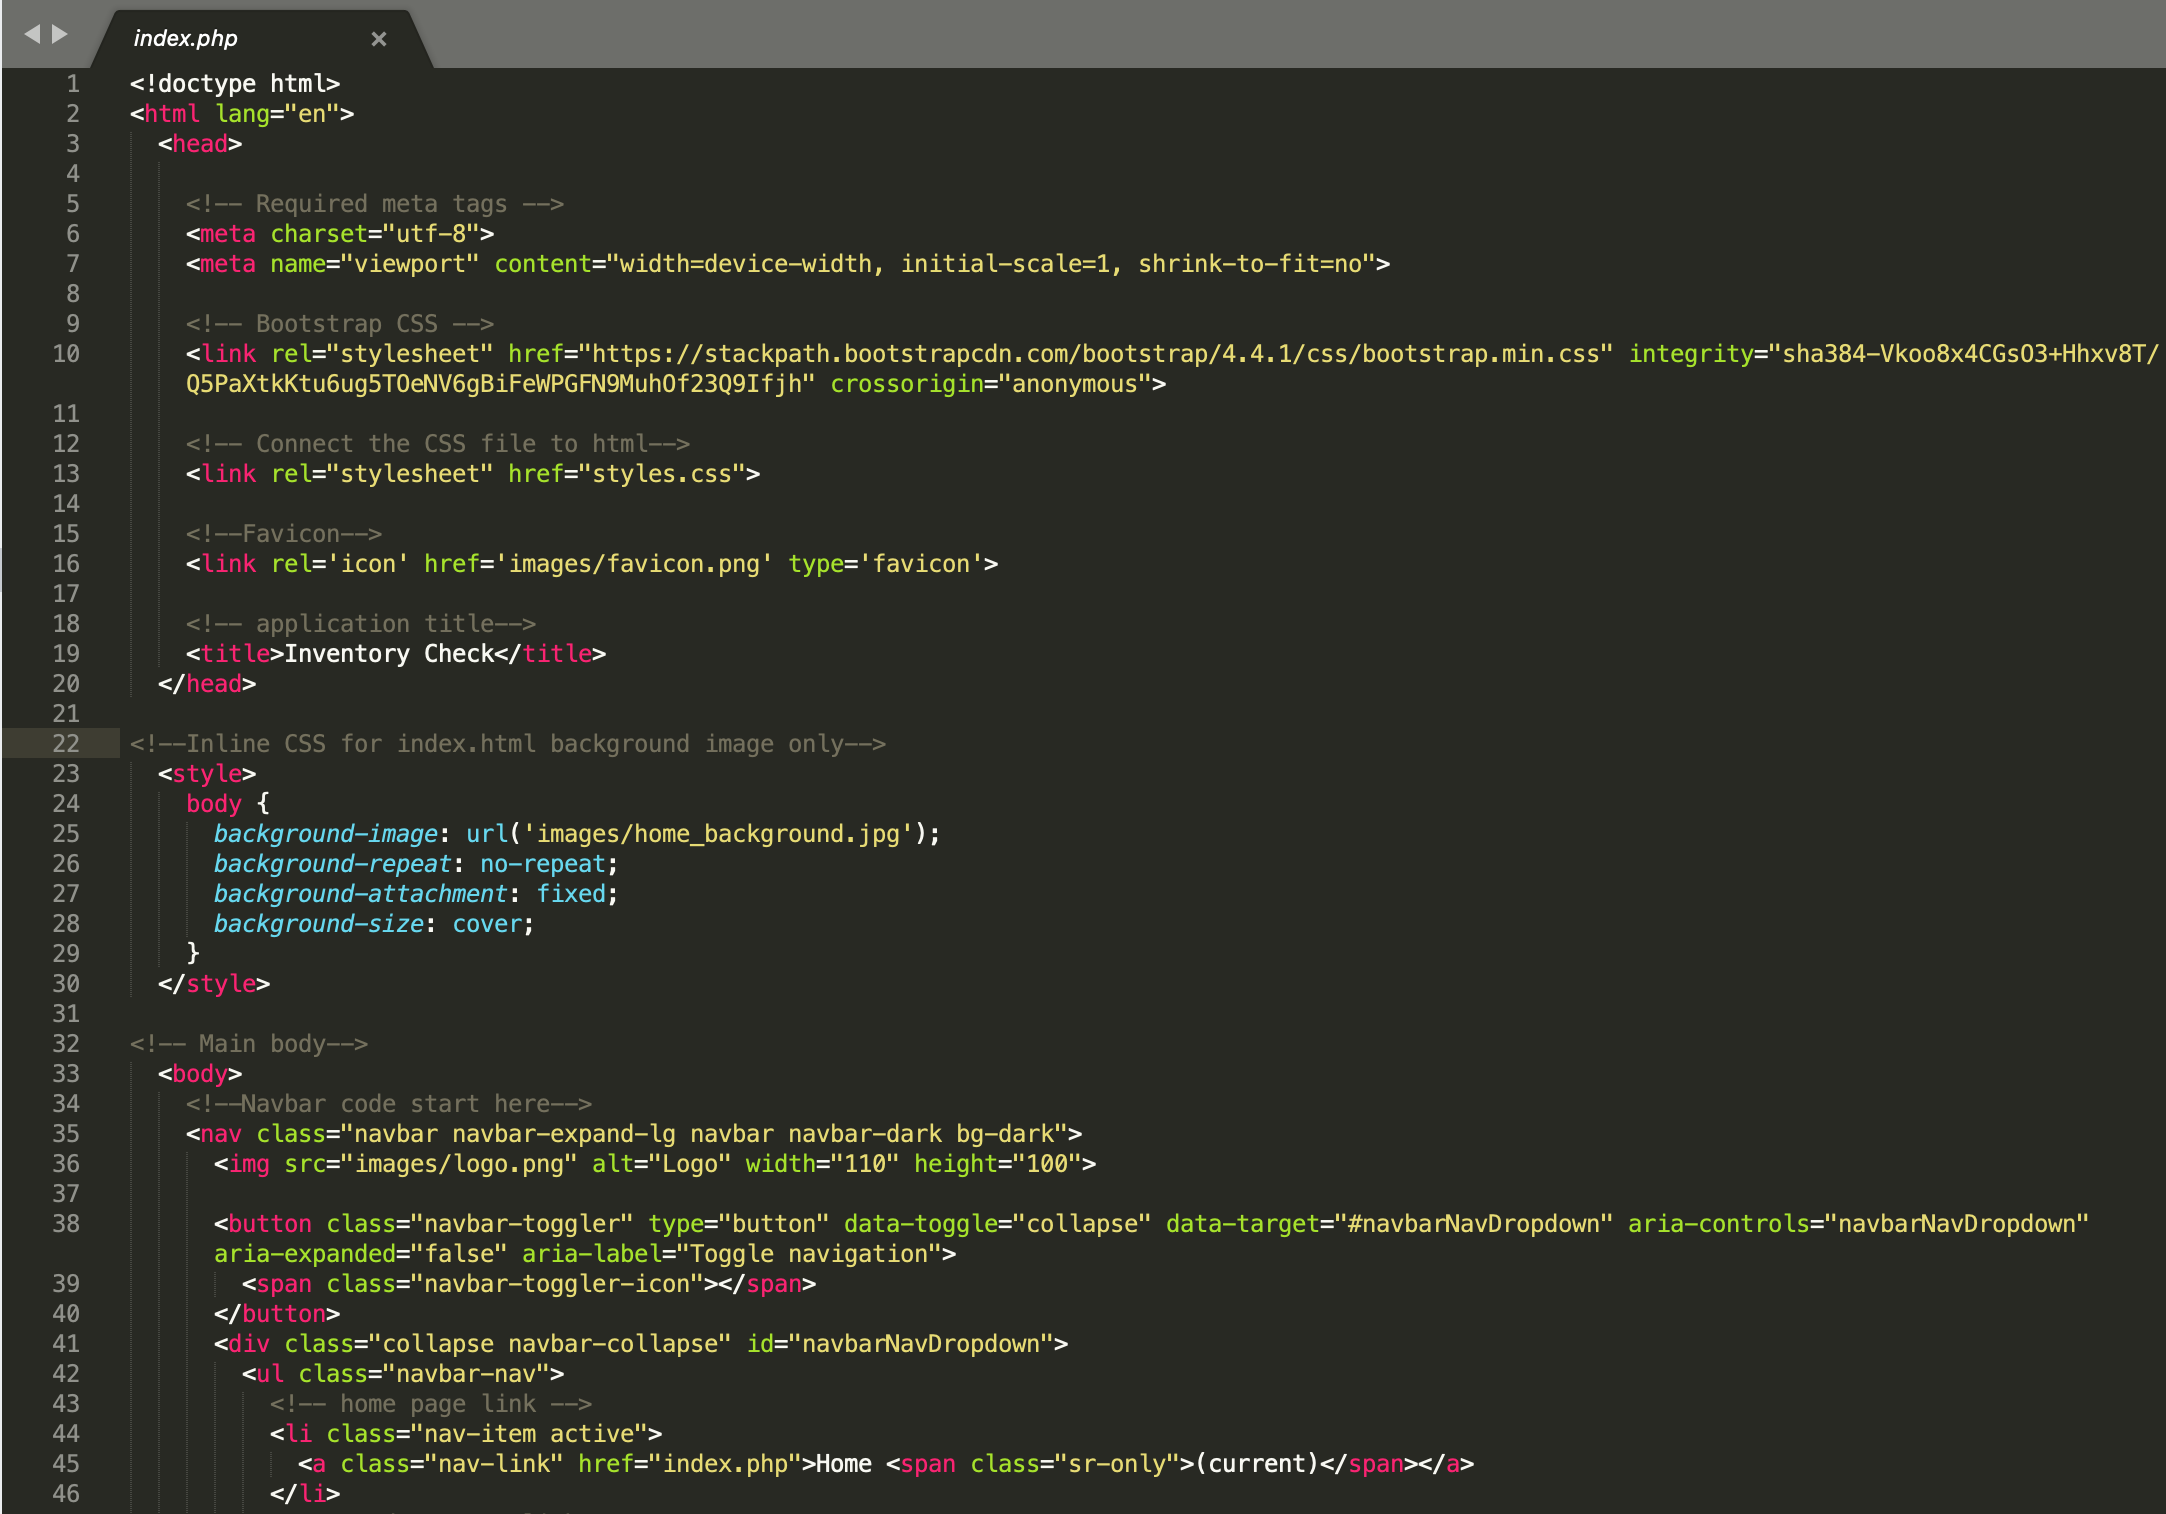
\includegraphics[scale=0.33]
    {implement_image/html.png}
    \caption{Example of HTML code}
    \label{fig:Example of HTML code}
\end{figure}

\subsection{CSS}
It is a style sheet language that is used for how documents are presented to users with different styles, layout, etc. Figure 4.2 shows the CSS code used in the index.php page to make the login form center-right.

\begin{figure}[H]
\centering
    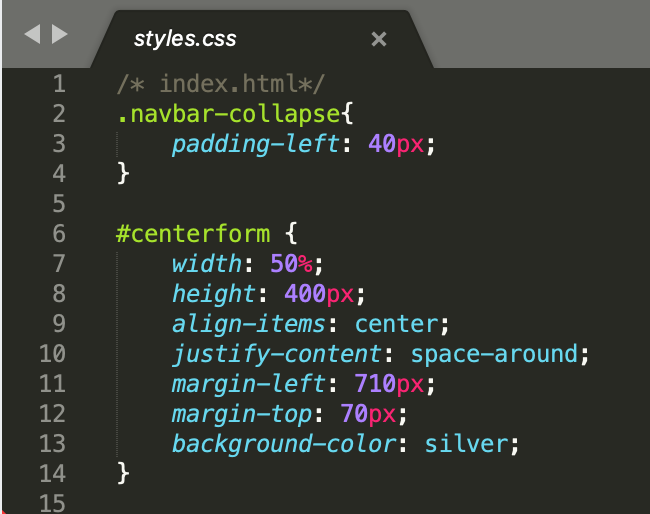
\includegraphics[scale=0.56]
    {implement_image/css.png}
    \caption{Example of CSS code}
    \label{fig:Example of CSS code}
\end{figure}

\subsection{JavaScript/jQuery}
It is a scripting language that enables the user to implement complex features on the web pages such as interactive maps, 2D or 3D graphics, alert dialog, etc. I have used this language to make the interactive map and executing the contact form. Figure 4.3 shows the JavaScript code which will execute once the user clicks on the submit button on the contact form.

\begin{figure}[H]
\centering
    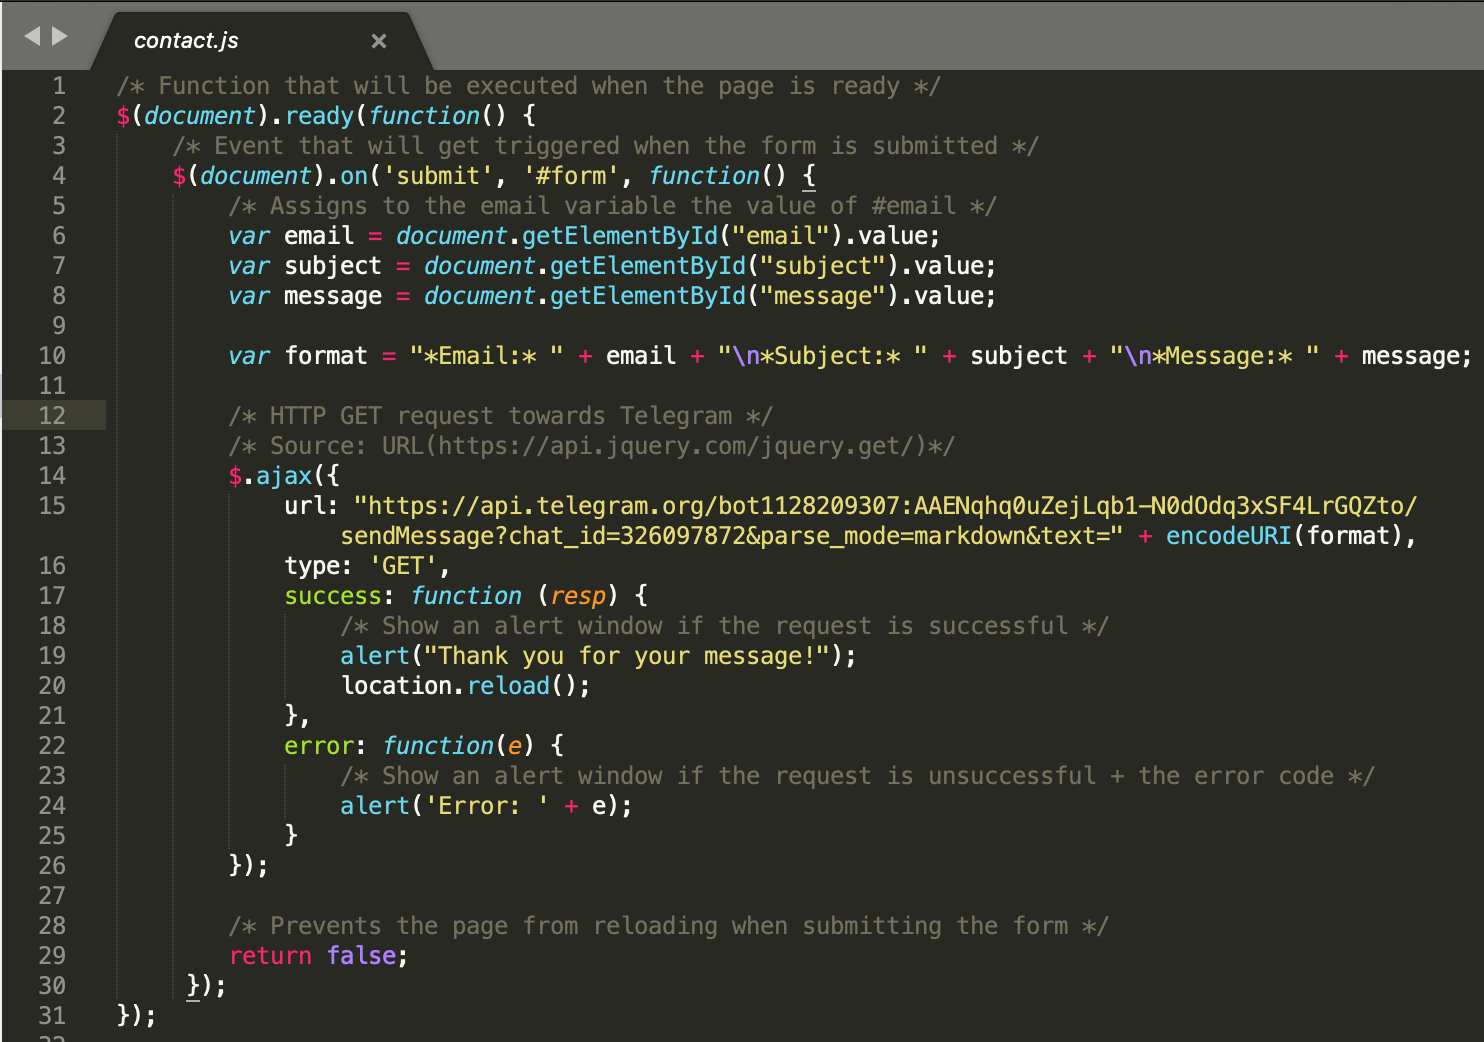
\includegraphics[scale=0.5]
    {implement_image/javascript.png}
    \caption{Example of JavaScript code}
    \label{fig:Example of JavaScript code}
\end{figure}

\section{PHP}
PHP is largely used by the back-end server and executes an important feature throughout the system. I have used PHP to view all products, edit products, add products, search products, delete the product, and analyse the product which will be shown in chart form using google chart library. It is a direct communication gateway between the server-side and client-side databases.

\subsection{Database Connection}
In order for my database to interact with the system, I need to establish a connection between the database and PHP script. Figure 4.4 is the code that connect my PHP script to XAMPP server.
\begin{figure}[H]
\centering
    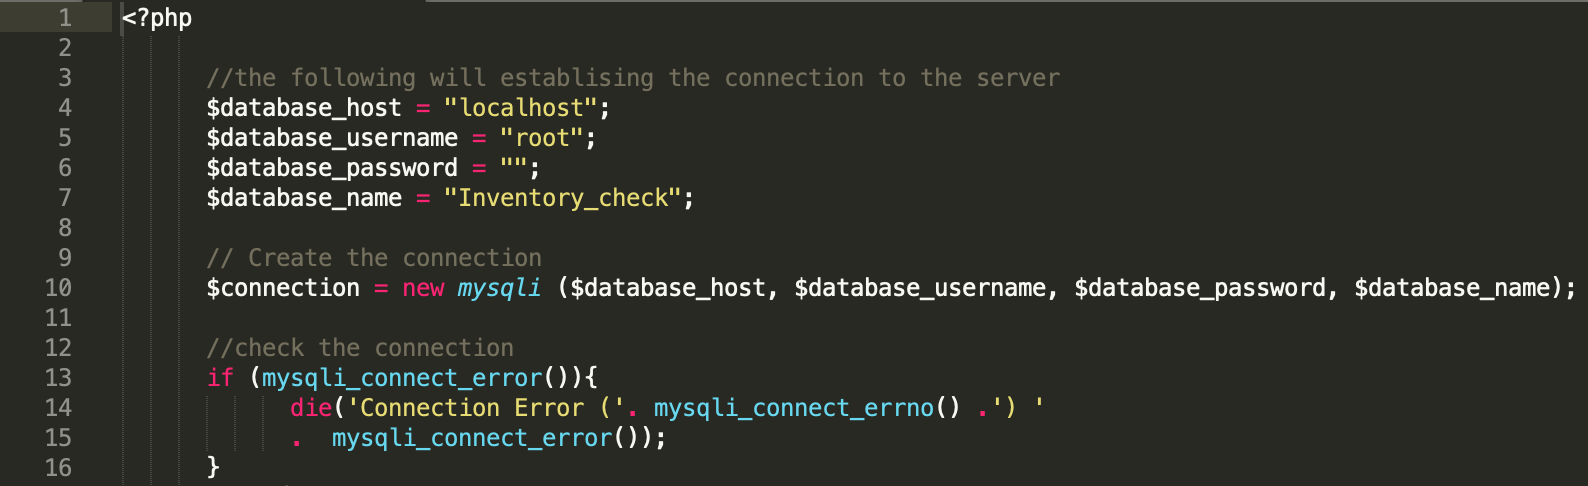
\includegraphics[scale=0.48]
    {implement_image/databaseconnection.png}
    \caption{ Connection to the server}
    \label{fig:Connection to the server}
\end{figure}

\subsection{View all product}
It is essential that the user can view all the products that are in the database as a list format. Firstly, it will establish the connection between the database and the PHP script. After that, it will execute the query ("SELECT * FROM add product ORDER BY time DESC";) which will gather all the suitable data from add product table. Once the data is gathered, the PHP echo will display all the data in descending order by time to the user screen(Figure 4.5 - line 107 to 117). This will show the most recent product add in the database first. If the database has no record to display then it will show the following message "There are no data in the database" in line 134 - Figure 4.5.

\begin{figure}[H]
\centering
    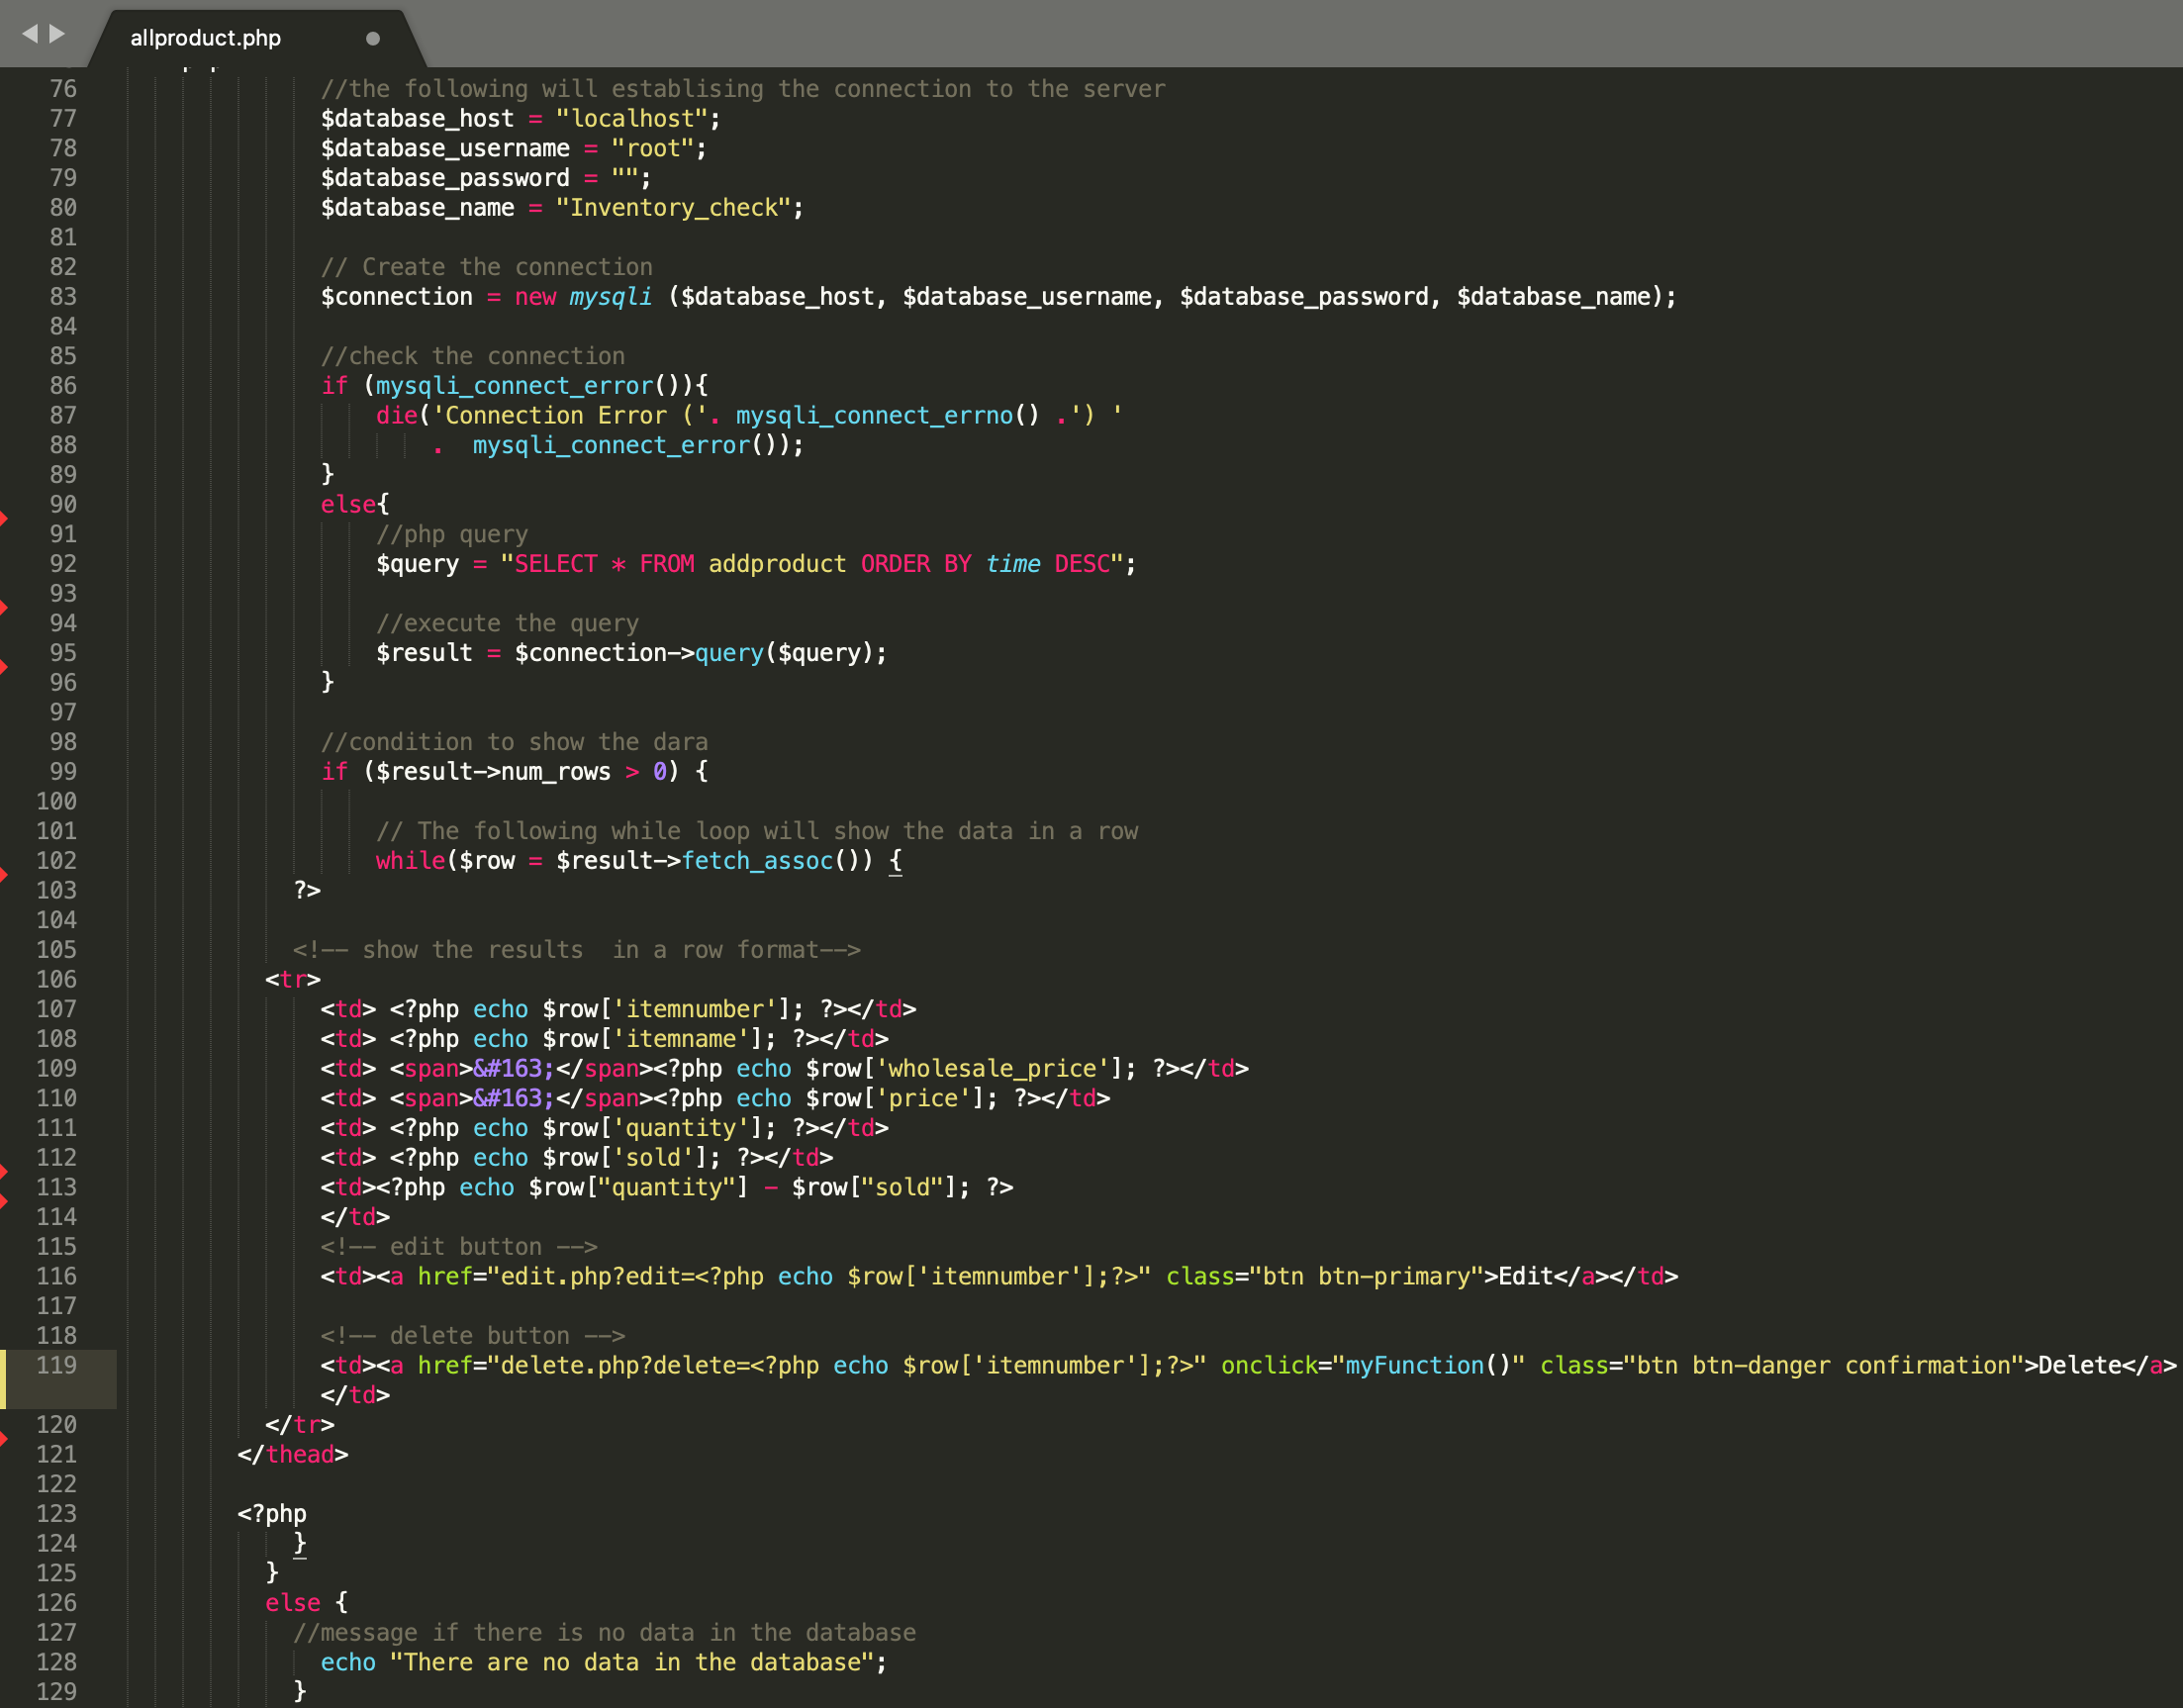
\includegraphics[scale=0.35]
    {implement_image/viewallproduct.png}
    \caption{allproduct.php}
    \label{fig:allproduct.php}
\end{figure}

\subsection{Add product}
The first most important thing for this system to have is to add the product in the database. This was created by using the POST method to transfer information through HTTP header and store data in the database. Figure 4.6, Line 42(if(isset(\$\_POST[ 'submit']))) is a if statement which will execute when the user click on submit button from the add product HTML form. It will then run the query(line 52 to 53) that will insert the data in add product table in the database and display the message if the record has been successfully inserted or not. Once the record has been successful insert, the user can add more records using the same HTML form. 

\begin{figure}[H]
\centering
    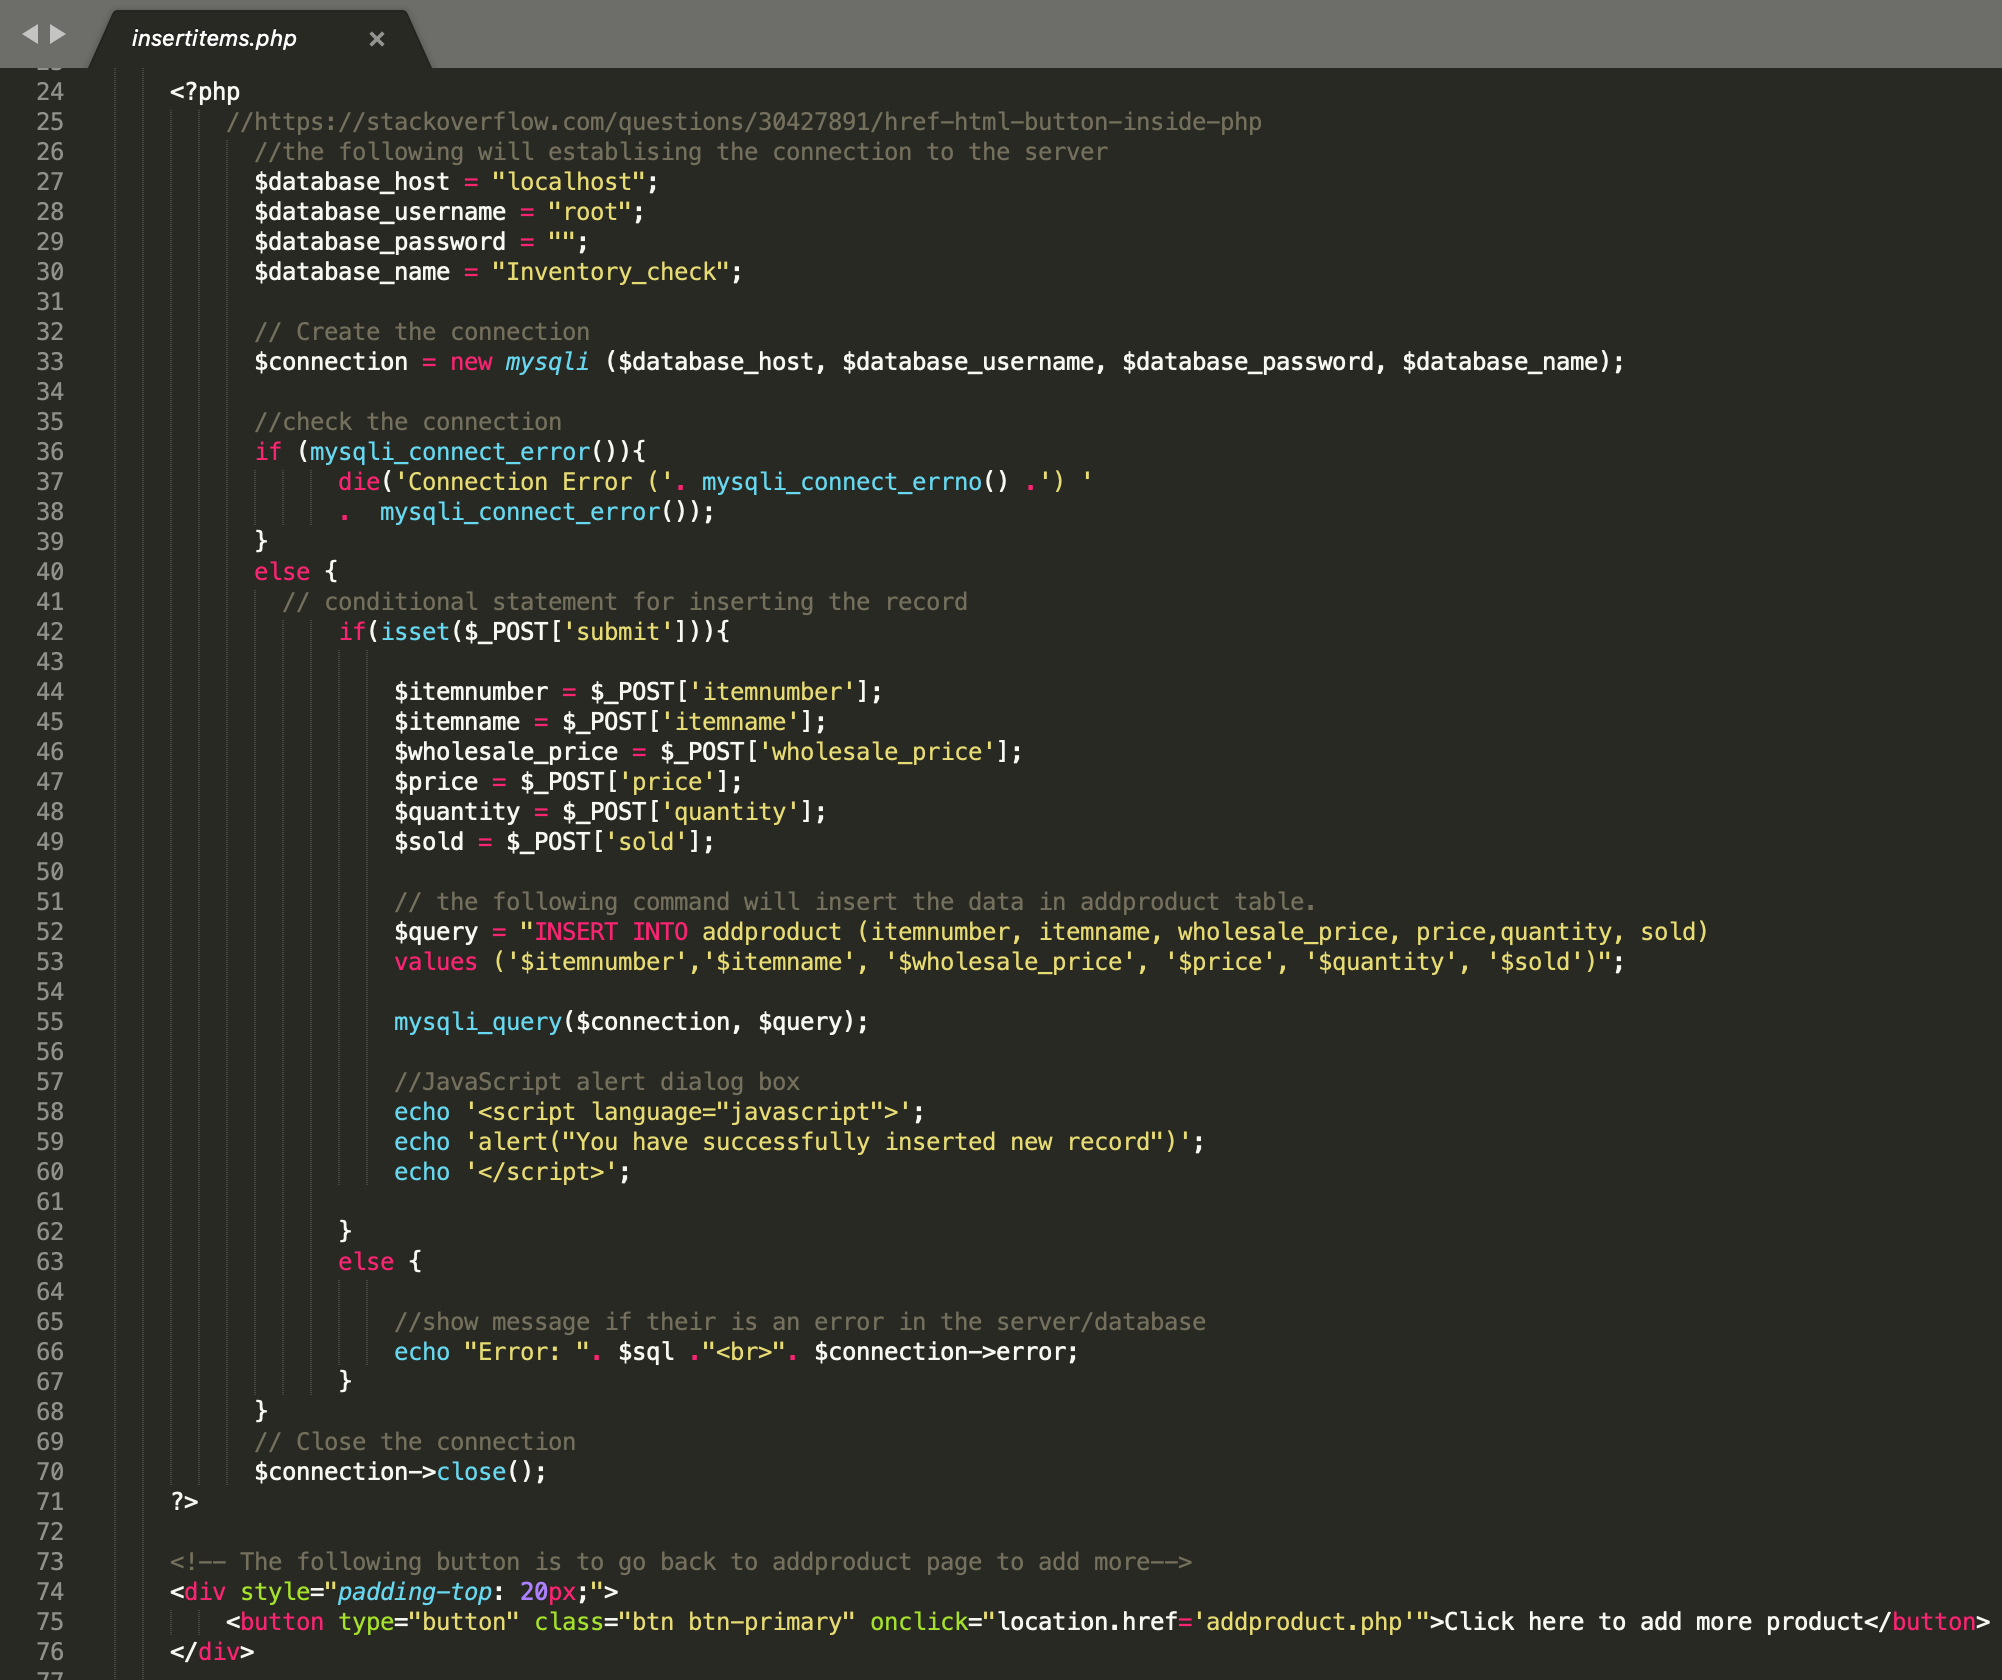
\includegraphics[scale=0.37]
    {implement_image/addproduct.png}
    \caption{insertitem.php}
    \label{fig:insertitem.php}
\end{figure}

\subsection{Edit  product}
The edit.php will get the existing data to show in the edit form. This was done by using the GET method that uses item number as id. The while loop in figure 4.7 will fetch all the data in the form and allow the user to edit the record. After changing the record user click on update button which will than use POST method (if(isset(\$\_POST['update']))) to update the data into the database. Once the record is updated the system will take the user to allproduct.php page using the header method(line 53).

\begin{figure}[H]
\centering
    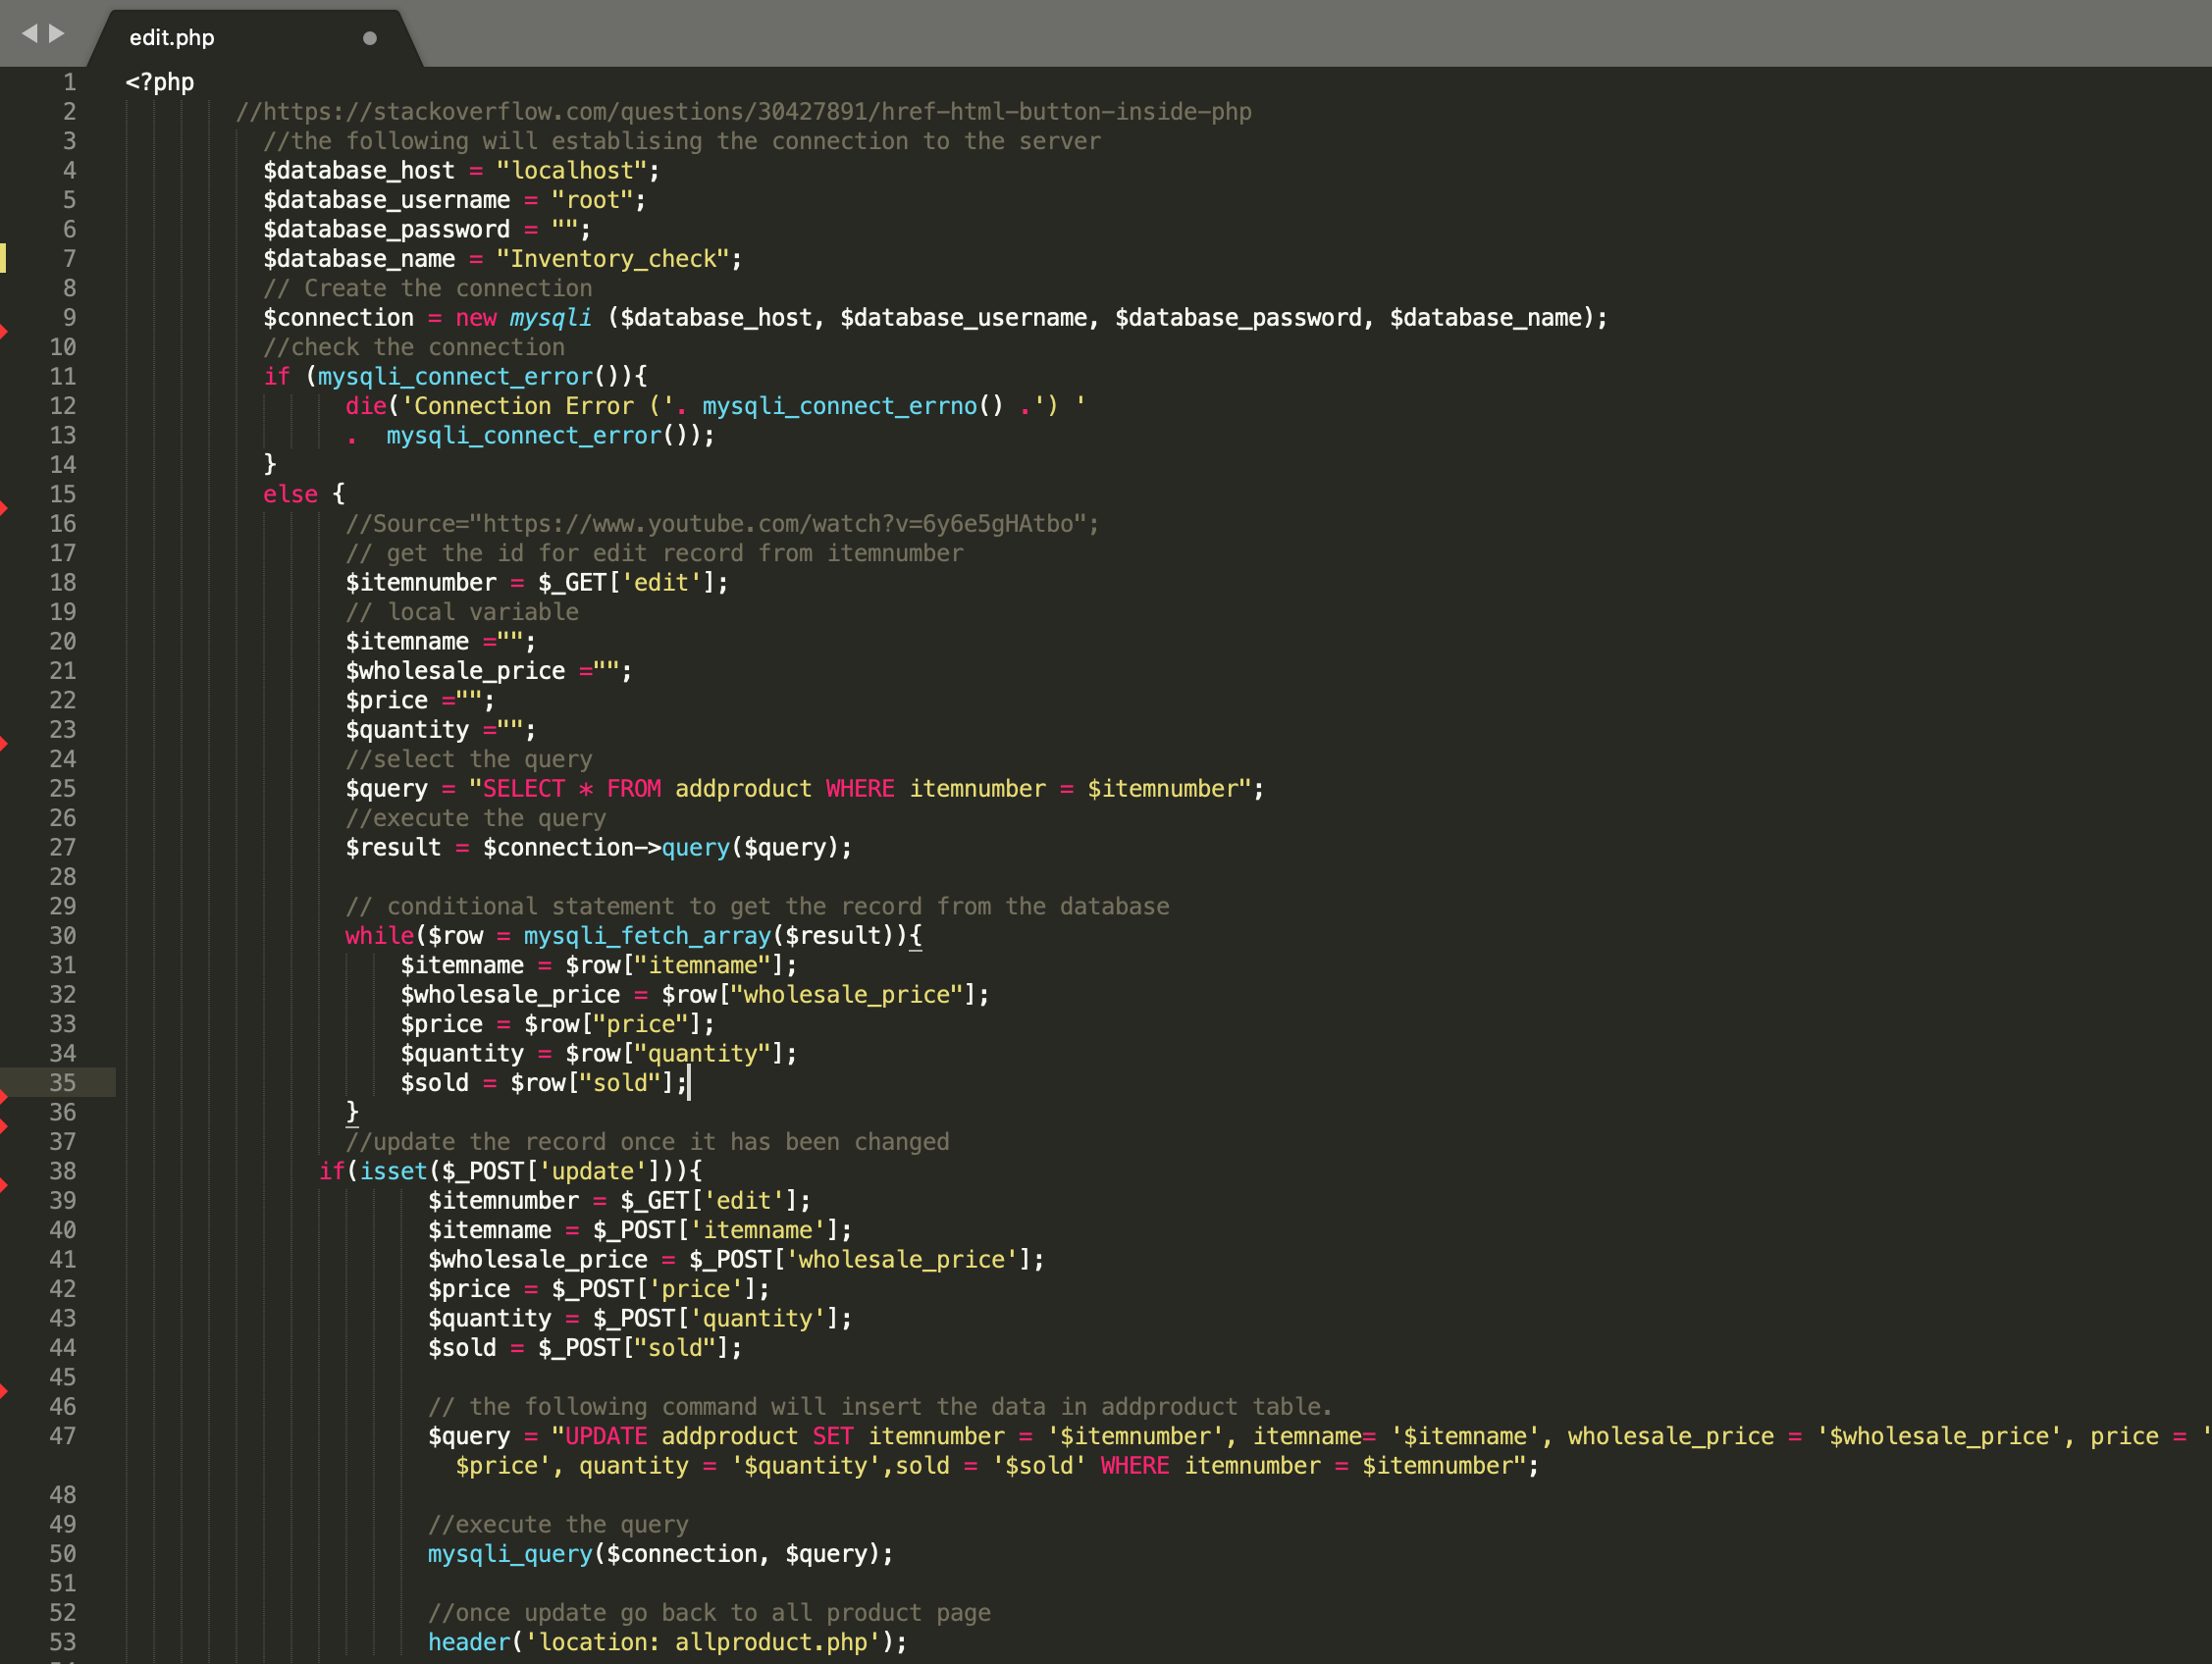
\includegraphics[scale=0.34]
    {implement_image/editproduct.png}
    \caption{edit.php}
    \label{fig:edit.php}
\end{figure}

\subsection{Delete product}
The delete.php will delete the entire record from the database. This was done by using the GET method where I have to use the item number as id. Based on item number it will look for a record in the database and once the record is found it will run a query (DELETE FROM `addproduct` WHERE item number = \$itemnumber) where it will delete the record. After deleting the record, the page will be refresh using the header method in line 30.
\begin{figure}[H]
\centering
    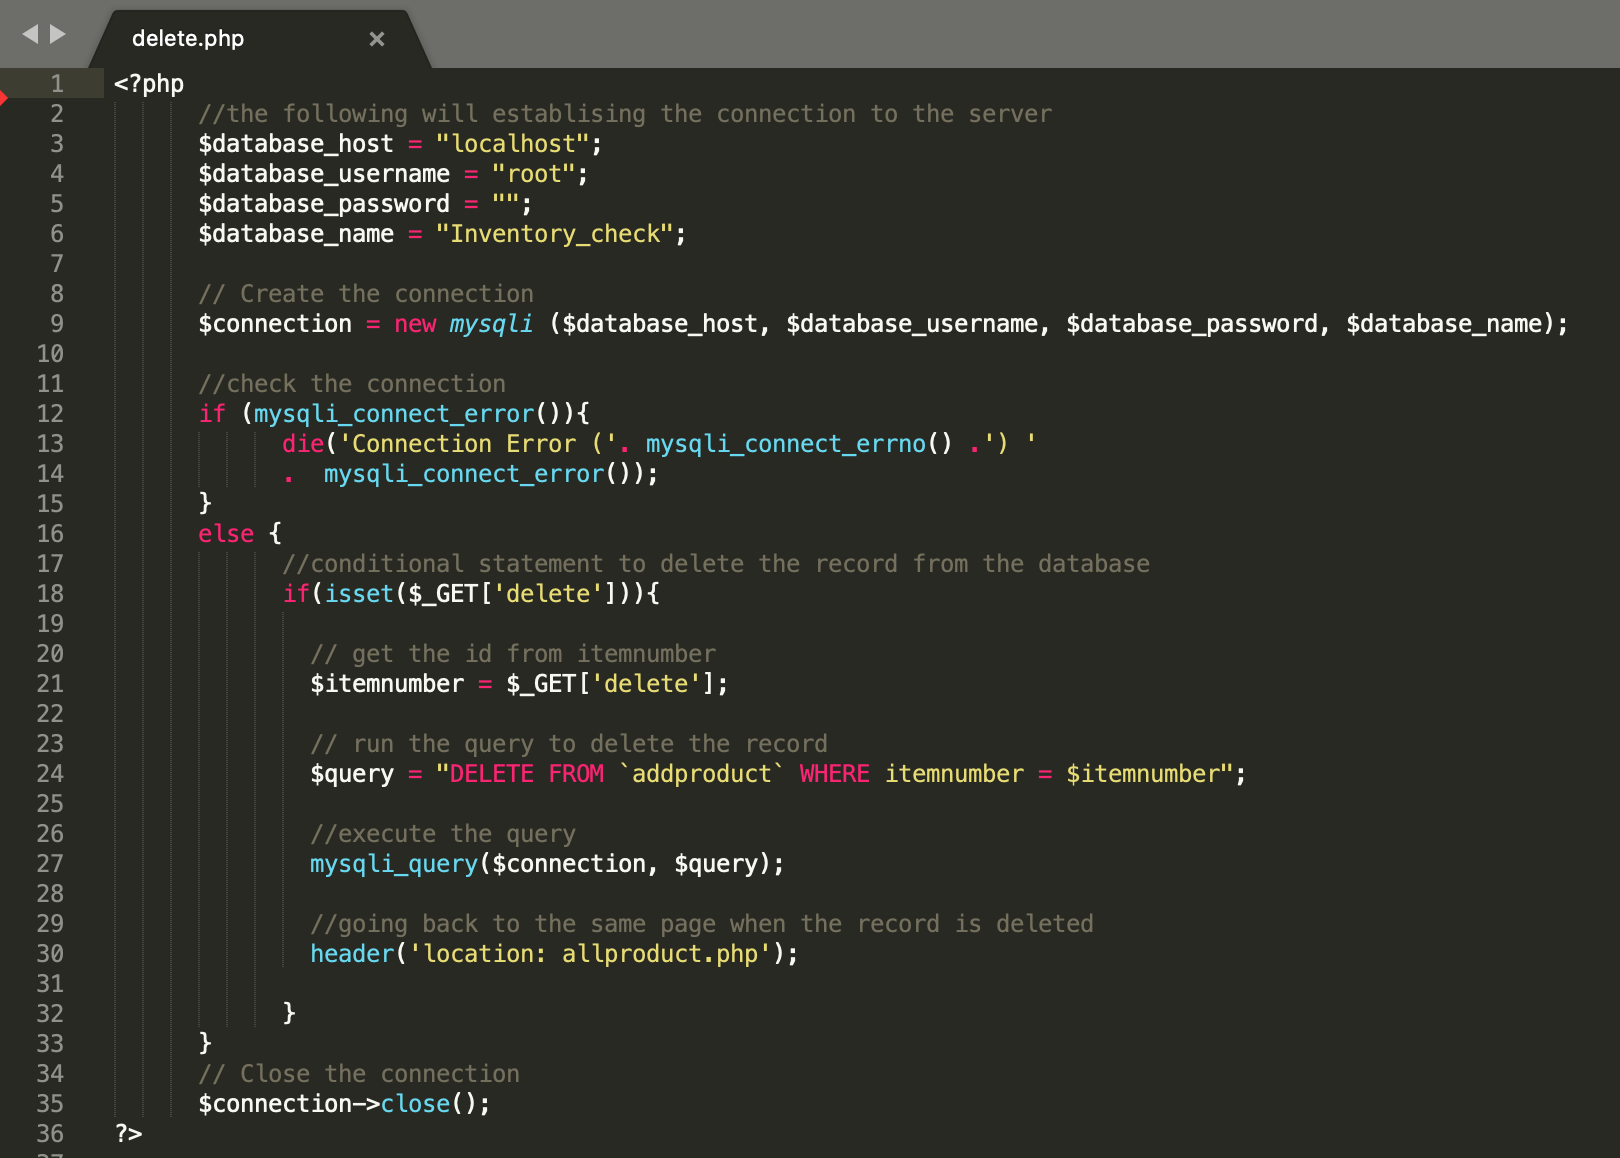
\includegraphics[scale=0.48]
    {implement_image/delete.png}
    \caption{delete.php}
    \label{fig:delete.php}
\end{figure}

\subsection{Search product}
The user can able to search the specific product using the item name or item name. This is one of the main features to add in the system as there will be more than a thousand products in the database and users cannot look for every record therefore by making the search functionality will be easier to look for exact data. This was built by using the GET method where (if(isset(\$\_GET['word']))) if statement will look for the record based on what user have input in the search field. It will then run the query in line 68 (Figure 4.9) and retrieve the result.

\begin{figure}[H]
\centering
    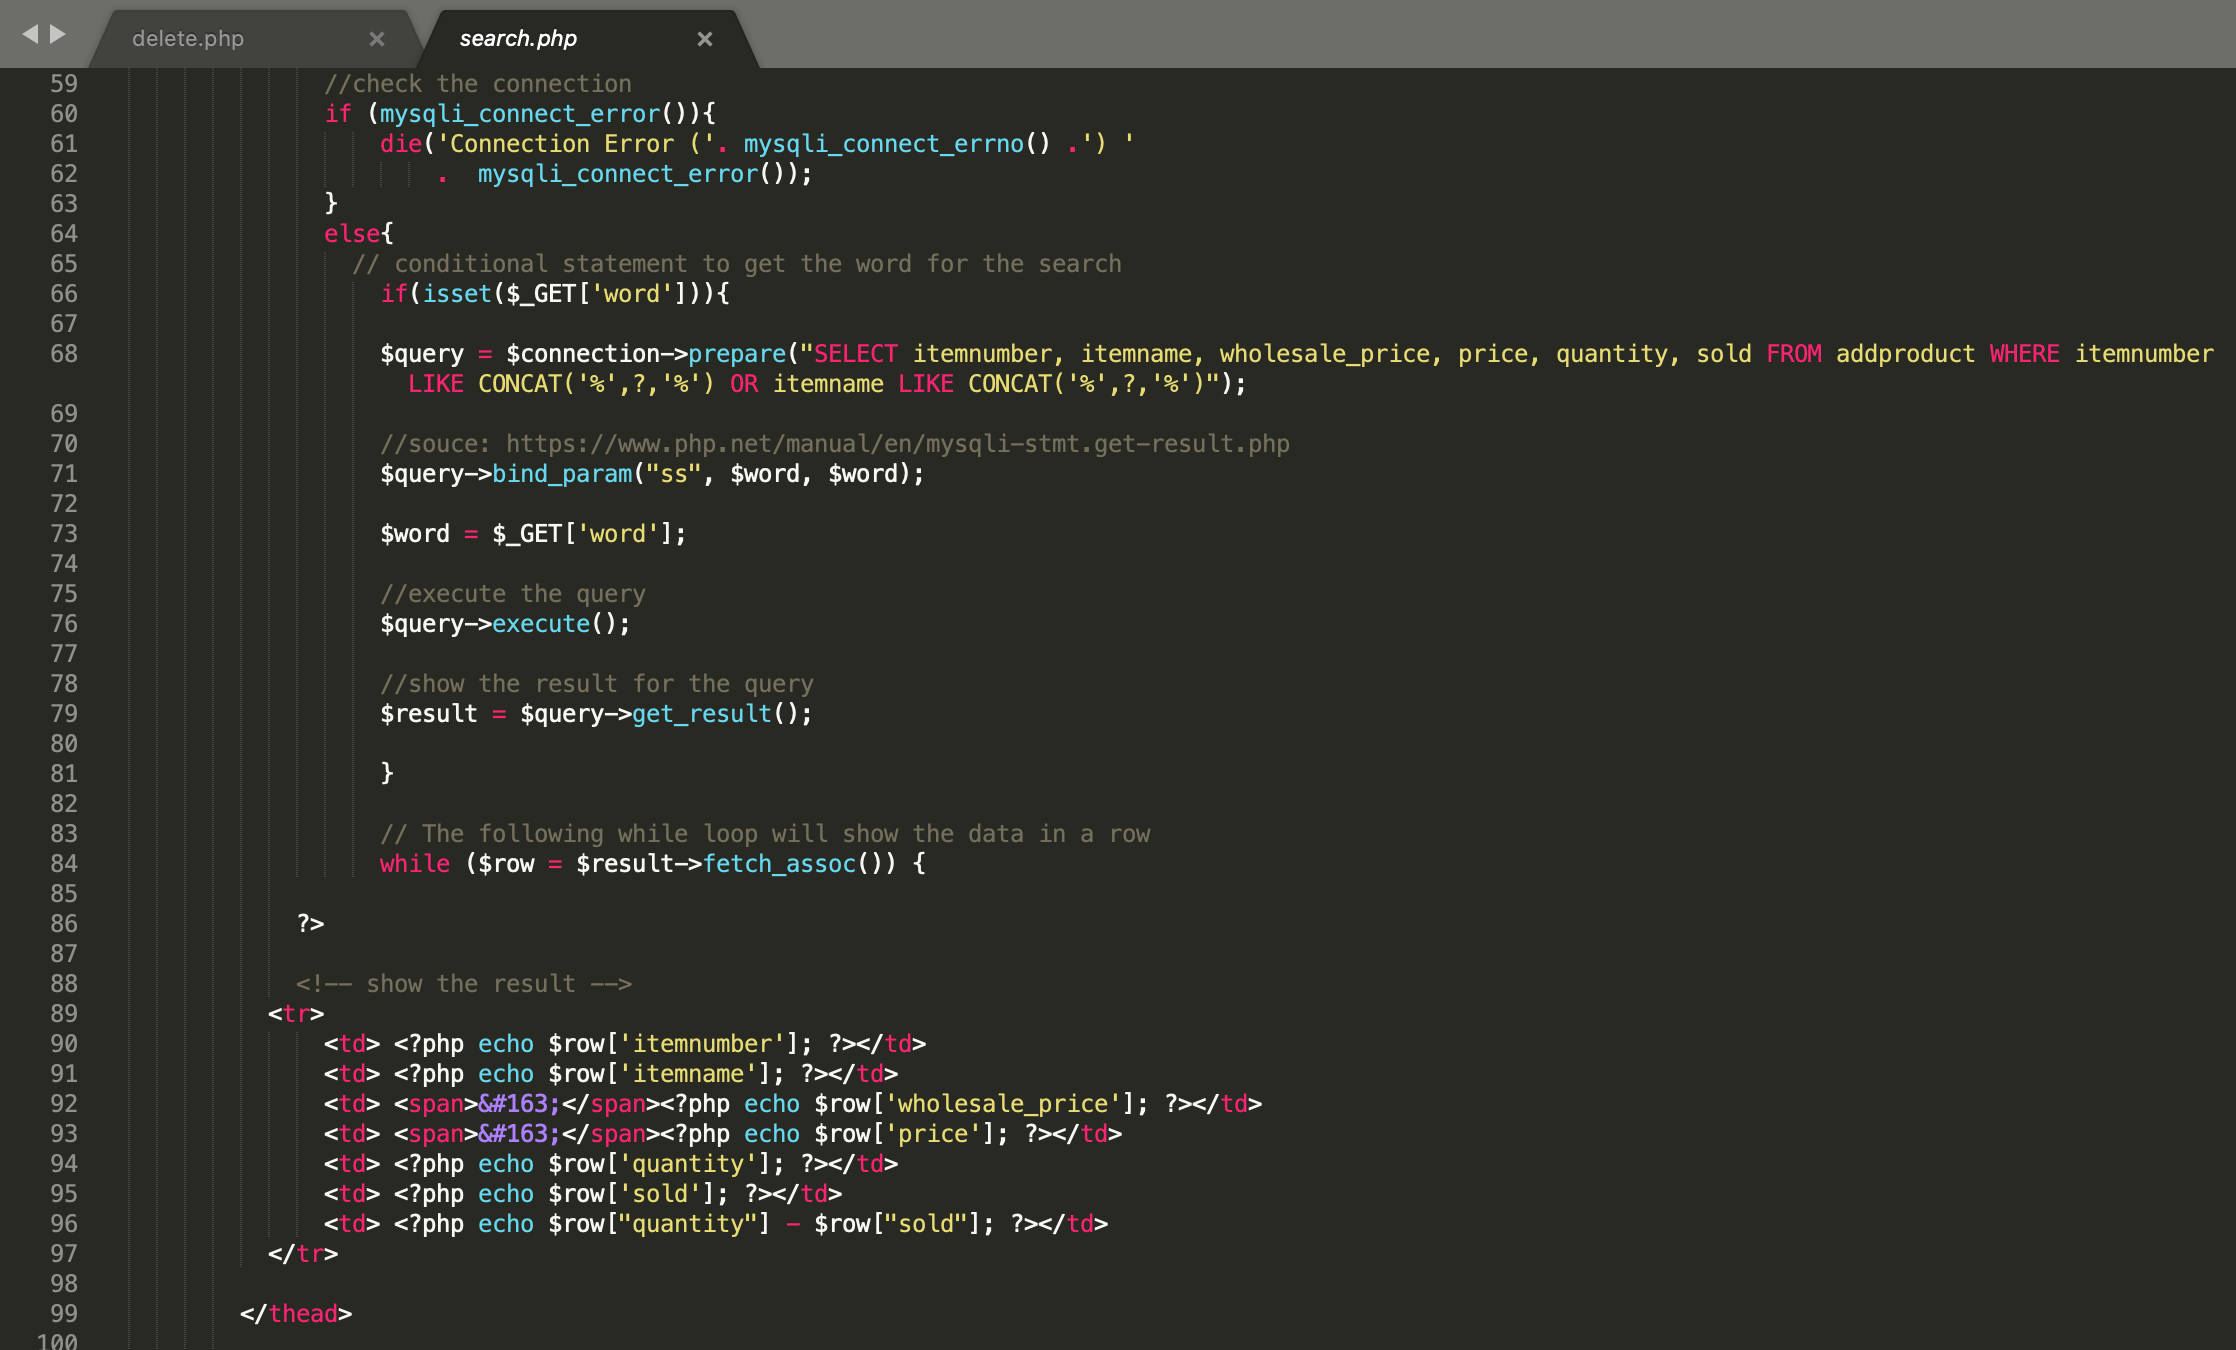
\includegraphics[scale=0.34]
    {implement_image/search.png}
    \caption{search.php}
    \label{fig:search.php}
\end{figure}

\subsection{Analyse product}
In order to create a chart to analyse the data, I have used the google chart API that allows me to create a graphical chart from a database record. There is a number of different charts with this library such as line, spline, area, pie, table, bar charts, etc. In my system, I have used bar chart and table chart, where bar chart will show the number of sold time, ordered by ascending and table chart shows information about the total cost from the wholesale price, in-store price, profit between wholesale product/in-store and total sale on a sold item. Figure 4.10 (Line 93), fetch all the results from the database and convert those data in a chart format. 

\begin{figure}[H]
\centering
    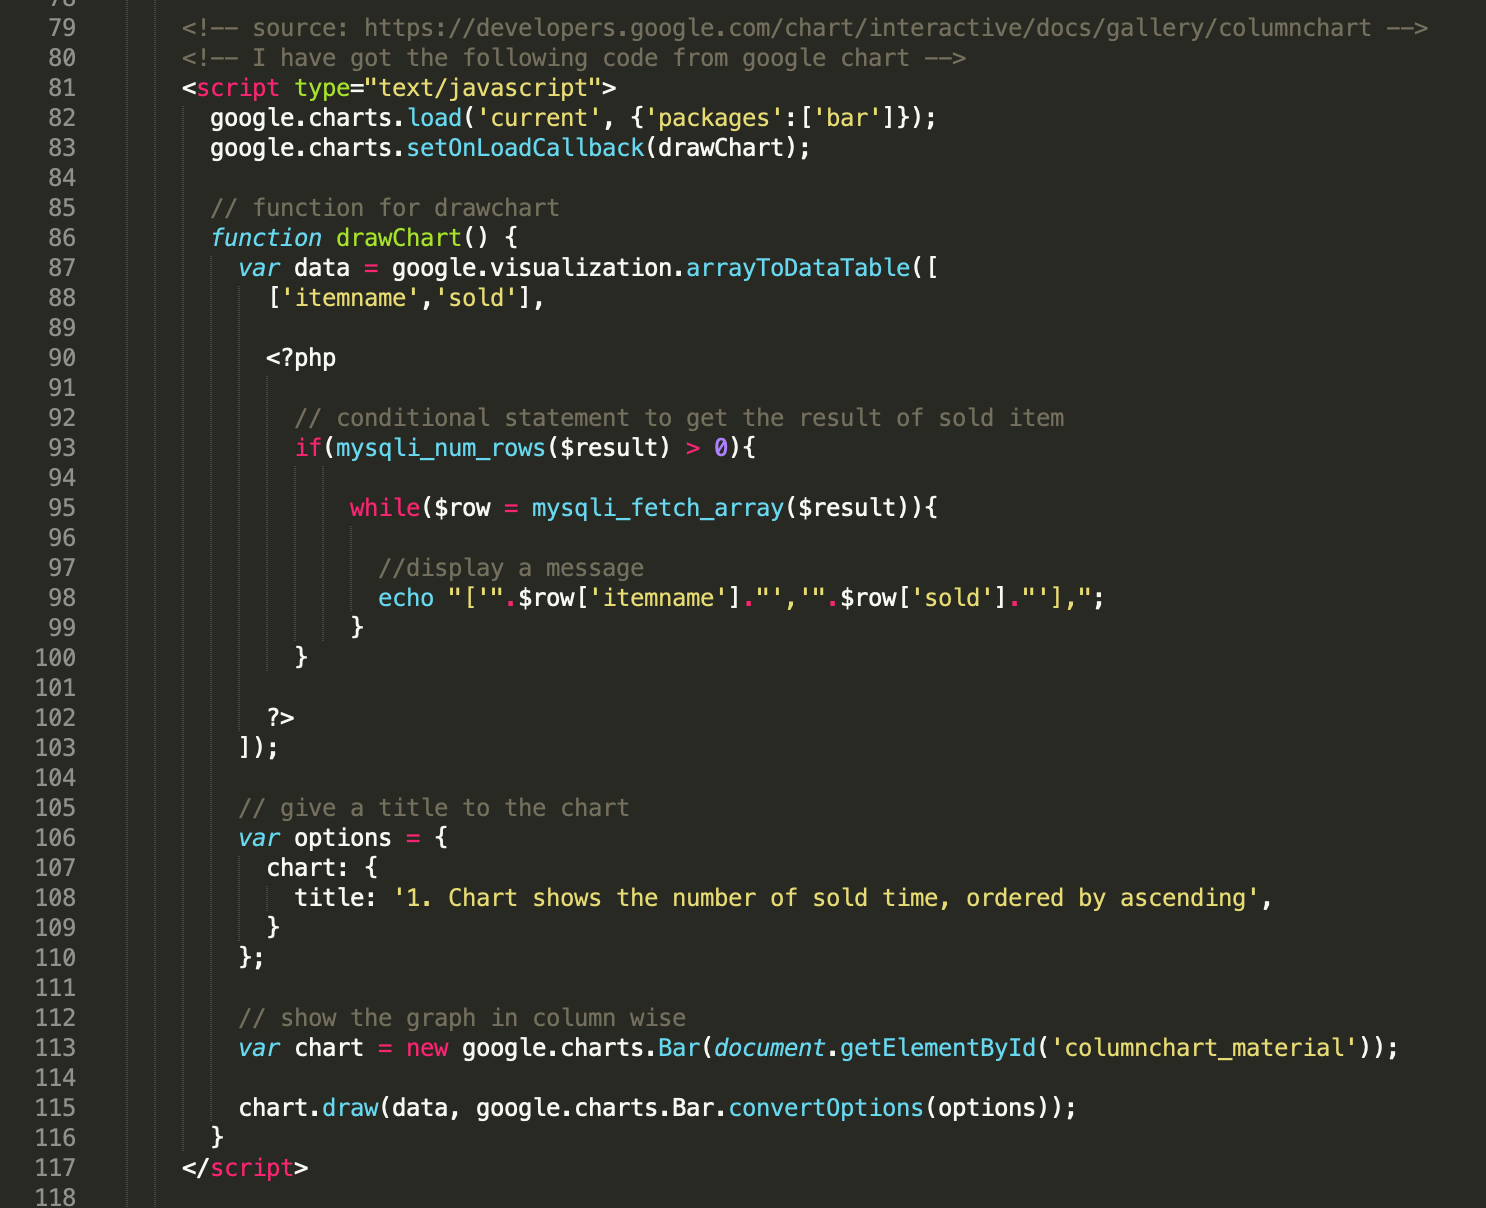
\includegraphics[scale=0.5]
    {implement_image/analyse.png}
    \caption{analystic.php}
    \label{fig:analystic.php}
\end{figure}

\section{MySQL}
The application use a back-end database which was implemented using MySQ L database. The following figures are the list of tables that has been used in the system.
\begin{figure}[H]
\centering
    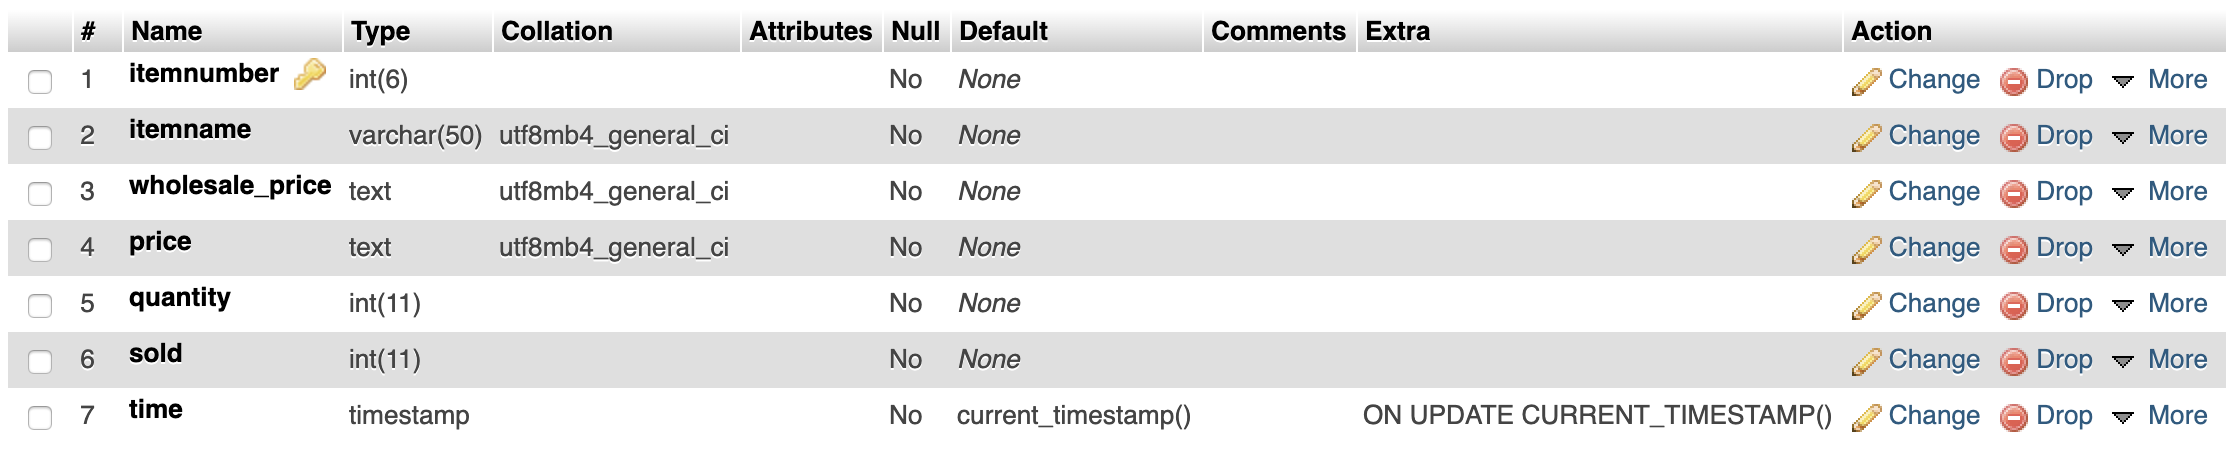
\includegraphics[scale=0.34]
    {implement_image/product.png}
    \caption{Product Table}
    \label{fig:Product Table}
\end{figure}

This feature has been implemented in the system yet but will be added in further development.
\begin{figure}[H]
\centering
    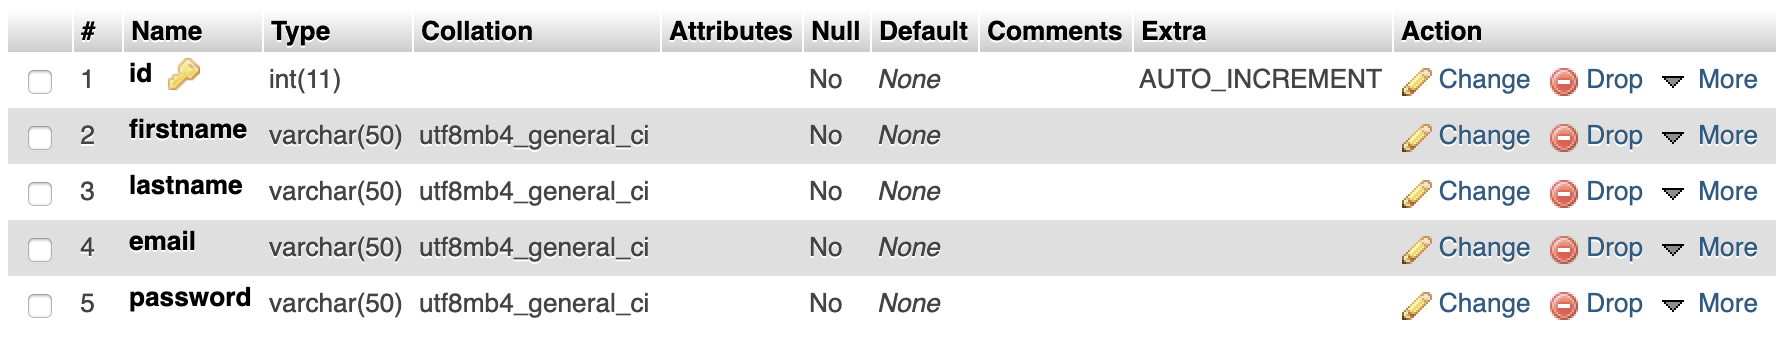
\includegraphics[scale=0.4]
    {implement_image/register.png}
    \caption{Register/Login Table}
    \label{fig:Register/Login Table}
\end{figure}


\section{Telegram API}
To make the contact form interact with the developer, I have used the Telegram API which will allow me to make a program that uses a telegram message for an interface. This means all the message submit in the contact form will be displayed in the telegram app. Inline 14-26, where HTTP GET the request toward telegram and show the alert when the message has successfully sent in line 19. In line 10 is the format that enables how to show the message in the telegram app.

\begin{figure}[H]
\centering
    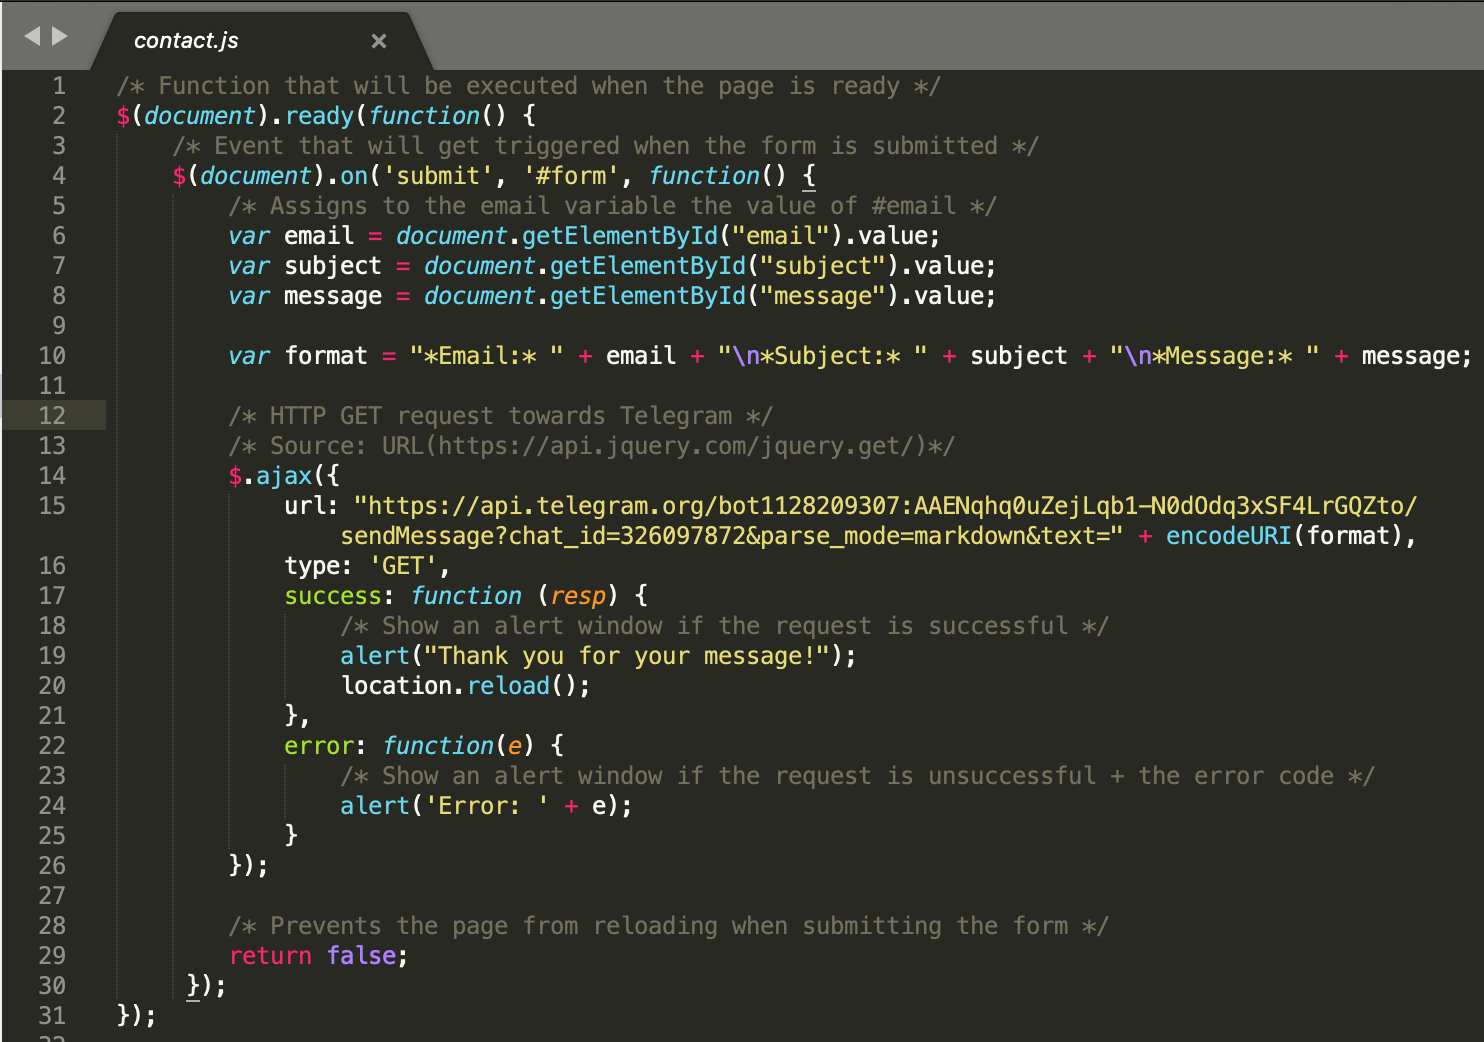
\includegraphics[scale=0.41]
    {implement_image/javascript.png}
    \caption{Example of API code}
    \label{fig:Example of API code}
\end{figure}

\section{Gantt Chart}
A Gantt chart is mainly used for managing the project and is one of the best ways of showing activities displayed against time. It is an effective tool when managing a complex project with many dependencies. I have used this methodology to manage my time during the project so I can complete all the tasks that I have given to myself on time.  I had shared this chart with my supervisor so he will know what task I have finished and what task I am currently working on. In figure 4.14 has the number of activities along with the time scale. Each activity is represented by a task name, duration, start date, end date, and comment if I missed any of the deadlines. This will ensure that I need to complete each activity within the time that I have specified in the chart, Therefore I can deploy the project on time.

\begin{figure}[H]
\centering
    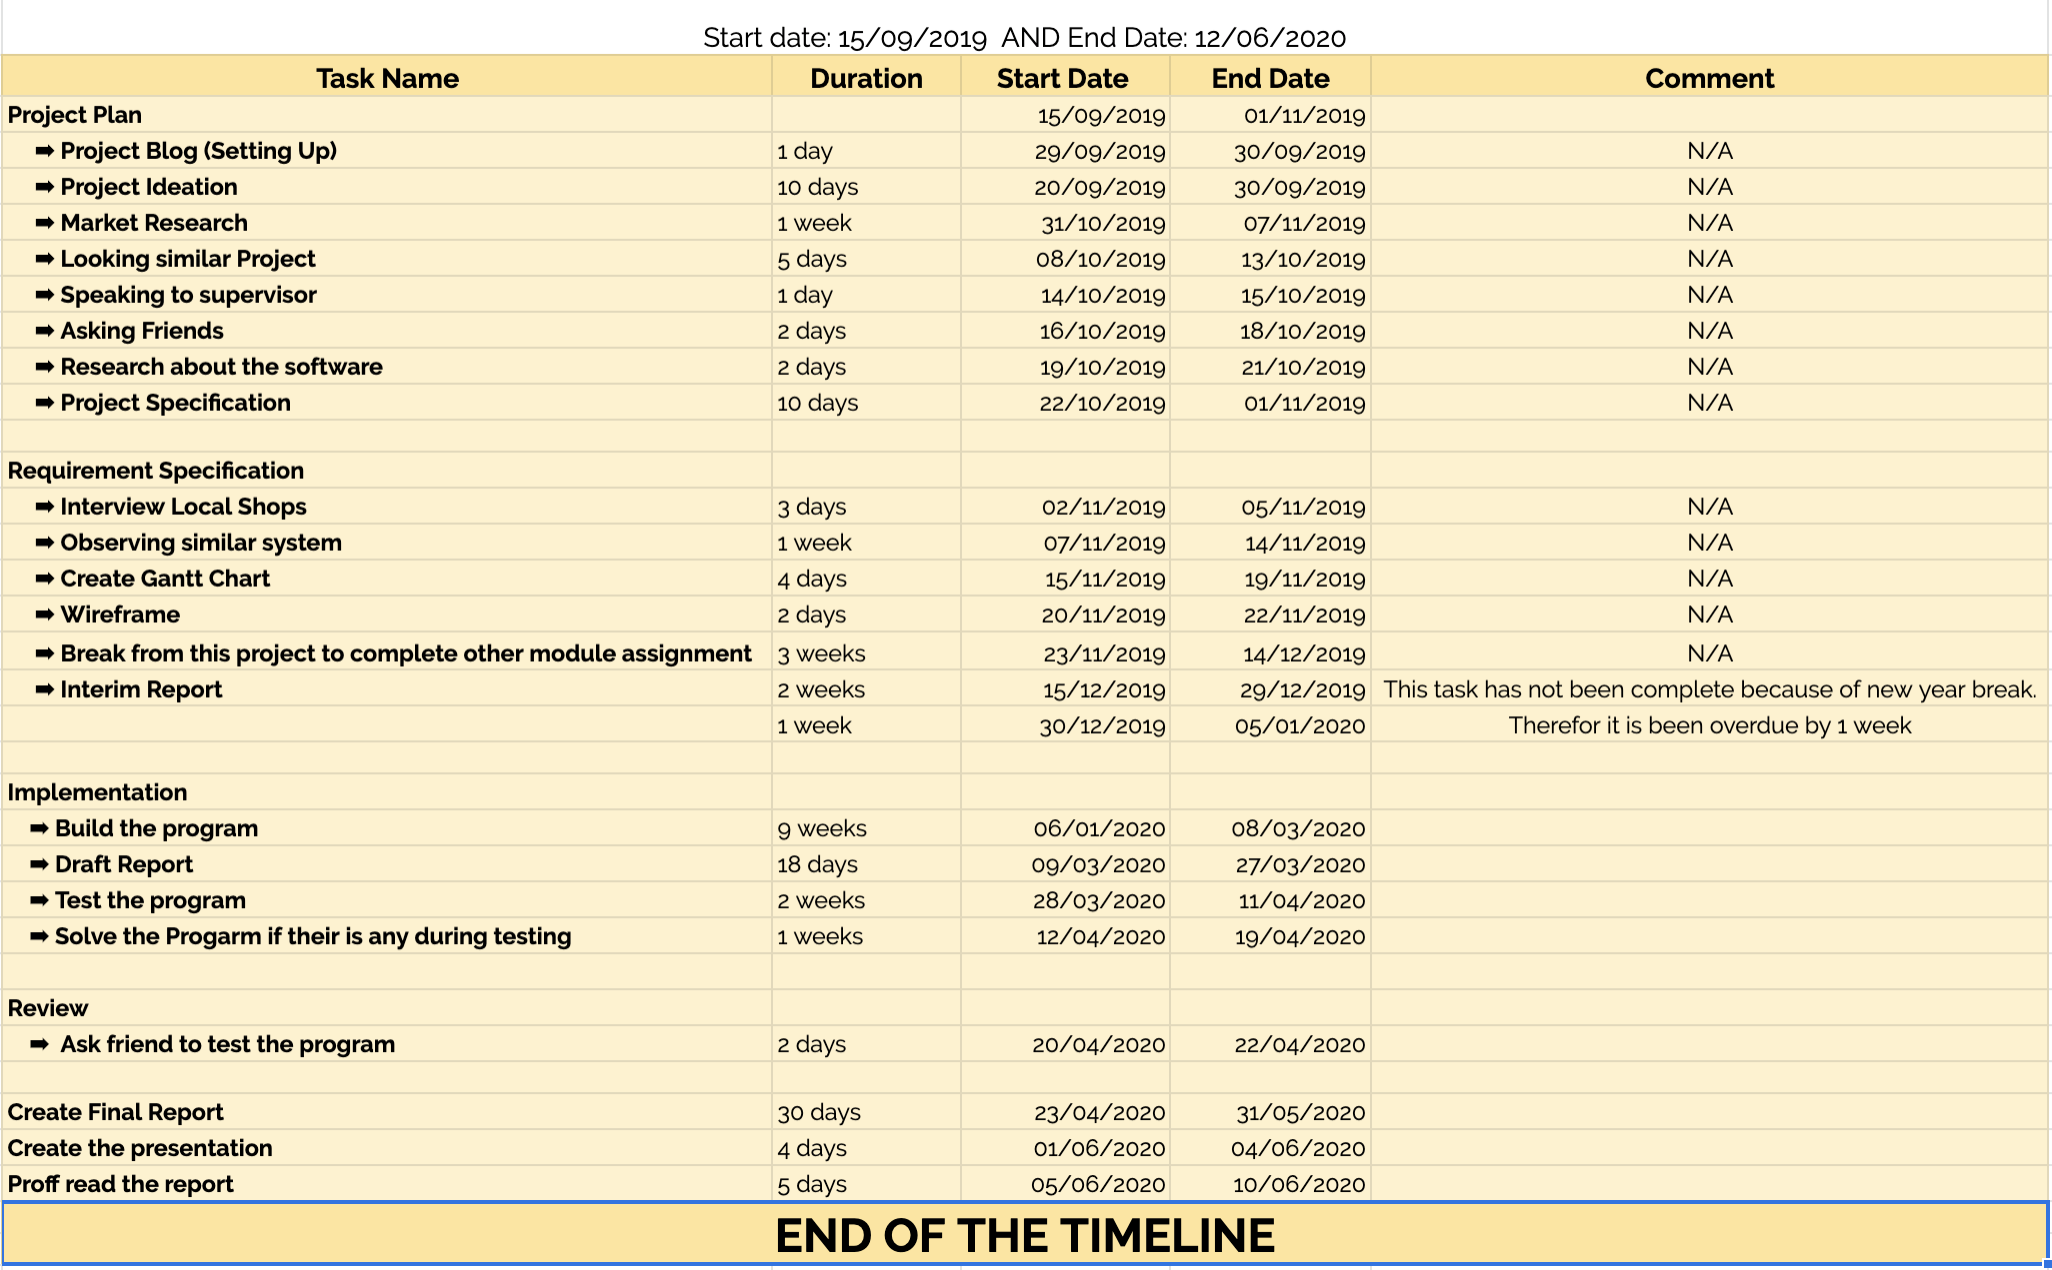
\includegraphics[scale=0.37]
    {ganttchart.png}
    \caption{Gantt Chart}
    \label{fig:Gantt Chart}
\end{figure}


